%


\documentclass[twoside]{article}
\setlength{\oddsidemargin}{0.25 in}
\setlength{\evensidemargin}{-0.25 in}
\setlength{\topmargin}{-0.6 in}
\setlength{\textwidth}{6.5 in}
\setlength{\textheight}{8.5 in}
\setlength{\headsep}{0.75 in}
\setlength{\parindent}{0 in}
\setlength{\parskip}{0.1 in}

%
% ADD PACKAGES here:
%

\usepackage{amsmath,amsfonts,graphicx}

%
\newcounter{lecnum}
\renewcommand{\thepage}{\thelecnum-\arabic{page}}
\renewcommand{\thesection}{\thelecnum.\arabic{section}}
\renewcommand{\theequation}{\thelecnum.\arabic{equation}}
\renewcommand{\thefigure}{\thelecnum.\arabic{figure}}
\renewcommand{\thetable}{\thelecnum.\arabic{table}}

%
% The following macro is used to generate the header.
%
\newcommand{\lecture}[4]{
   \pagestyle{myheadings}
   \thispagestyle{plain}
   \newpage
   \setcounter{lecnum}{#1}
   \setcounter{page}{1}
   \noindent
   \begin{center}
   \framebox{
      \vbox{\vspace{2mm}
    \hbox to 6.28in { {\bf EE302 - Feedback Systems
	\hfill Spring 2019} }
       \vspace{4mm}
       \hbox to 6.28in { {\Large \hfill Lecture #1 \hfill} }
       \vspace{2mm}
       \hbox to 6.28in { {\it Lecturer: #2 \hfill } }
      \vspace{2mm}}
   }
   \end{center}
   \markboth{Lecture #1}{Lecture #1}

   \vspace*{4mm}
}
%
\renewcommand{\cite}[1]{[#1]}
\def\beginrefs{\begin{list}%
        {[\arabic{equation}]}{\usecounter{equation}
         \setlength{\leftmargin}{2.0truecm}\setlength{\labelsep}{0.4truecm}%
         \setlength{\labelwidth}{1.6truecm}}}
\def\endrefs{\end{list}}
\def\bibentry#1{\item[\hbox{[#1]}]}

%Use this command for a figure; it puts a figure in wherever you want it.
%usage: \fig{NUMBER}{SPACE-IN-INCHES}{CAPTION}
\newcommand{\fig}[3]{
			\vspace{#2}
			\begin{center}
			Figure \thelecnum.#1:~#3
			\end{center}
	}
% Use these for theorems, lemmas, proofs, etc.
\newtheorem{theorem}{Theorem}[lecnum]
\newtheorem{lemma}[theorem]{Lemma}
\newtheorem{proposition}[theorem]{Proposition}
\newtheorem{claim}[theorem]{Claim}
\newtheorem{corollary}[theorem]{Corollary}
\newtheorem{definition}[theorem]{Definition}
\newenvironment{proof}{{\bf Proof:}}{\hfill\rule{2mm}{2mm}}

% **** IF YOU WANT TO DEFINE ADDITIONAL MACROS FOR YOURSELF, PUT THEM HERE:

\begin{document}

% Lecture Details
\lecture{15}{Asst. Prof. M. Mert Ankarali}

\par

\section{Nyquist Stability Criterion}

Nyquist stability criterion is another method to investigate 
the stability (absolute and relative) of a dynamical system
(feed-forward and feed-back). Its based on the frequency response
characteristics of a system.

\textbf{Definition:} A contour $\Gamma_s$ is a closed path with a direction
in a complex plane. 

\textbf{Remark:} A continuous function $F(s)$ maps a contour
$\Gamma_s$ in $s-$plane to another contour $\Gamma_{F(s)}$
in $F(s)$ plane. The figure below illustrates a clock-wise contour 
$\Gamma_s$ and its map $\Gamma_{F(s)}$ which is also clock-wise
in this example. 

\vspace{6 pt}

  \begin{minipage}[h]{1\linewidth}
    \begin{center}
      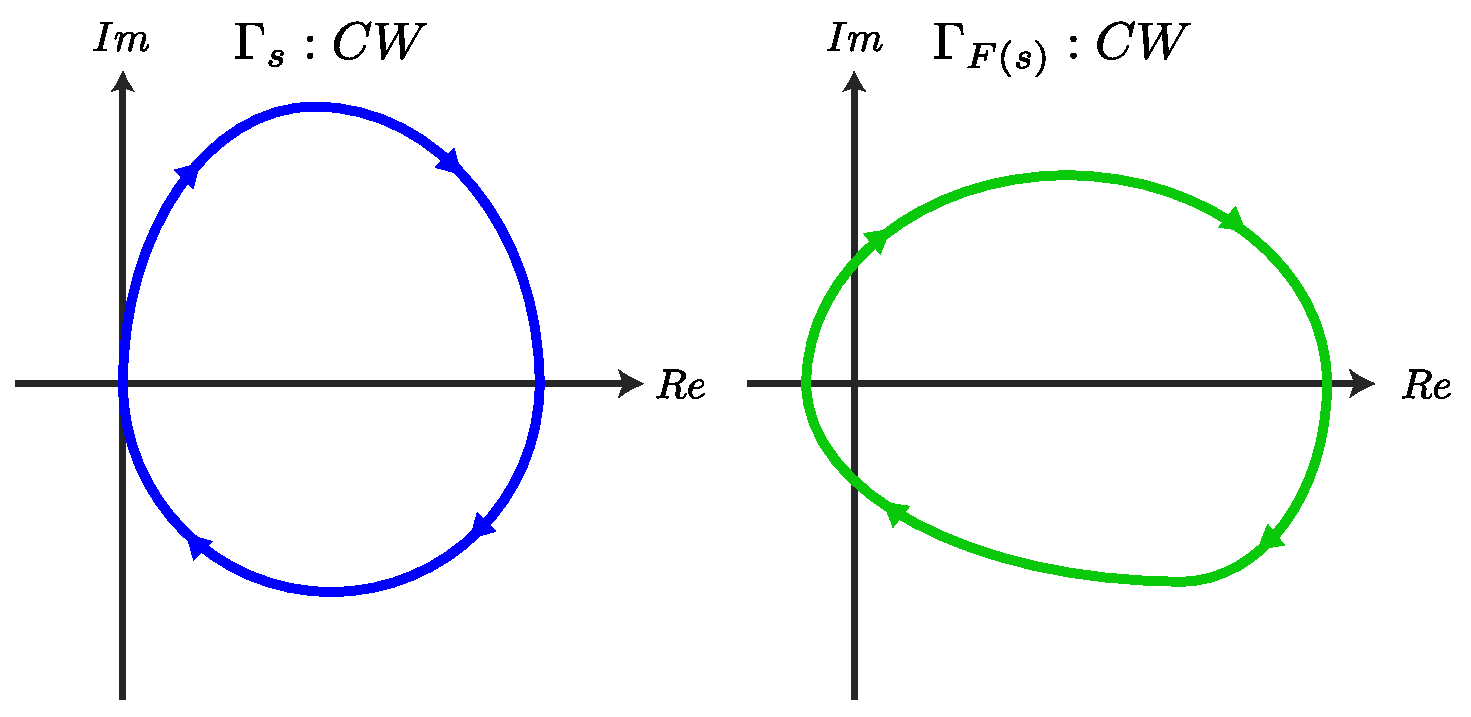
\includegraphics[width=0.80\textwidth]{cmap}
    \end{center}
  \end{minipage}

\vspace{6 pt}

\textbf{Theorem: Cauchy's Argument Principle}

Given $F(s) = \frac{N(s)}{D(s)}$ and a CW contour $\Gamma_s$ in $s-$ plane
which does not croes any zeros (roots of $N(s)$) or poles (roots of $D(s)$)
of $F(s)$, then the mapped contour $\Gamma_{F(s)}$ will encircle the
origin
%
\begin{align*}
  N &= Z  - P \quad \mathrm{times}
\\
  N &: \# \ \mathrm{CW} \ \mathrm{encirclements} \ \mathrm{of} \ \mathrm{origin}
\\
  Z &: \# \ \mathrm{zeros} \ F(s)
\\
  P &: \# \ \mathrm{poles} \ F(s)
\end{align*}

\subsection{Nyquist Stability Criterion for Feedforward Systems}

Let's assume that we want to analyze the stability of the following
input-output system

\vspace{6 pt}

  \begin{minipage}[h]{1\linewidth}
    \begin{center}
      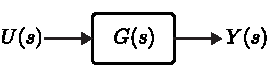
\includegraphics[width=0.3\textwidth]{sys}
    \end{center}
  \end{minipage}

\vspace{6 pt}

and we know that $G(s) = \frac{N(s)}{D(s)}$ has no zeros or poles on
the imaginary axis. Since we are intersted in finding the unstable
poles, Nyquist contour/path, $\Gamma_s$, is defined in a way that it covers the
whole open-right half plane. As illustrated in the Figure below, 
Nyquist contour is technically a half-circle for which the radius, $R
\to \infty$. After that, one can draw the Nyquist plot, which is the
mapped contour $\Gamma_{G(s)}$, and count the $\#$ of CW encirclements 
of the origin ($N$). Based on Cauchy's Argument Principle we know that
%
\begin{itemize}
  \item $P = Z - N$, where
  \item $N$: $\#$ CW encirclements of origin by $\Gamma_{G(s)}$
  \item $Z$: $\#$ zeros of $G(s)$ with positive real parts
  \item $P$: $\#$ poles of $G(s)$ with positive real parts
\end{itemize}

\vspace{6 pt}

  \begin{minipage}[h]{1\linewidth}
    \begin{center}
      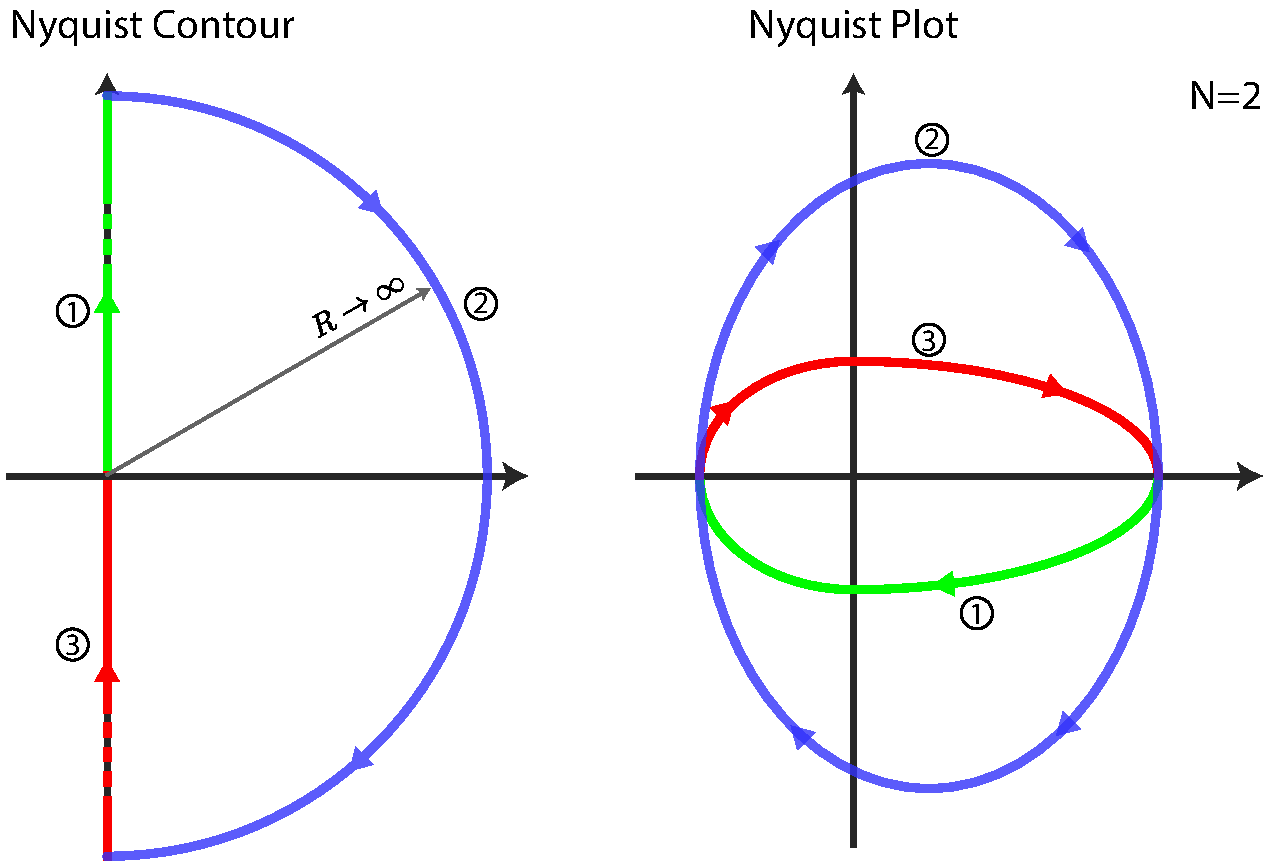
\includegraphics[width=0.9\textwidth]{nyq}
    \end{center}
  \end{minipage}

\vspace{6 pt}

In this example illustration $N = 2$, which implies that total number
of unstable poles of $G(s)$ is given by $P = Z + 2$, if $Z$,
i.e. number of zeros with positive real parts, is known than
we can compute number of unstable poles $P$. Alternatively, 
since in a feedforward system only denominator part determines
the stability, instead of $G(s)$, one can draw the Nyquist plot of 
$\bar{G}(s) = \frac{1}{D(s)}$.

\newpage

\textbf{Ex:} Let's analyze the feedforward stability of $G(s) =
\frac{s-1}{s+1}$ using Nyquist plot. 

\textbf{Solution:} Based on the Nyquist contour we have three major
paths
%
\begin{enumerate}
  \item This is the polar plot that we covered in the previous
    lecture, where we plot $G(j \omega)$, where $\omega : 0 \to \infty$
  \item This is the infinite radius circular path. In this case
   if we write $s$ in polar form, we get $s = R e^{j \theta}$
    where $R \to \infty$, and $\theta : \pi/2 \to -\pi/2$. Then 
   we can derive that  
   \begin{align*}
     & G \left( R e^{j \theta} \right) = 
     \frac{R e^{j \theta} - 1}{R e^{j \theta} + 1} 
     \approx \frac{R e^{j \theta}} {R e^{j \theta}}
       \\
    &\Rightarrow | G \left( R e^{j \theta} \right) | \approx 1
   \quad , \quad \angle [ G \left( R e^{j \theta} \right) ] \approx 0
   \end{align*}
  %
  In other words, this whole path in the Nyquist plot
  is concentrated around $1 + 0 j$ point in the complex plane.
  \item This path is the mapping of the negative imaginary axis, 
  i.e $G(-j \omega)$, where $\omega : \infty \to 0$. Obviously
  since $G(-j \omega)$ is complex conjugate of $G(j \omega)$
  this path is symmetric to the polar plot with respect to the 
  real axis. Note that direction of this path is reverse of the
  direction of the  polar plot.
\end{enumerate}

  If we follow the procedure, we obtain the following Nyquist plot. 

\vspace{6 pt}

  \begin{minipage}[h]{1\linewidth}
    \begin{center}
      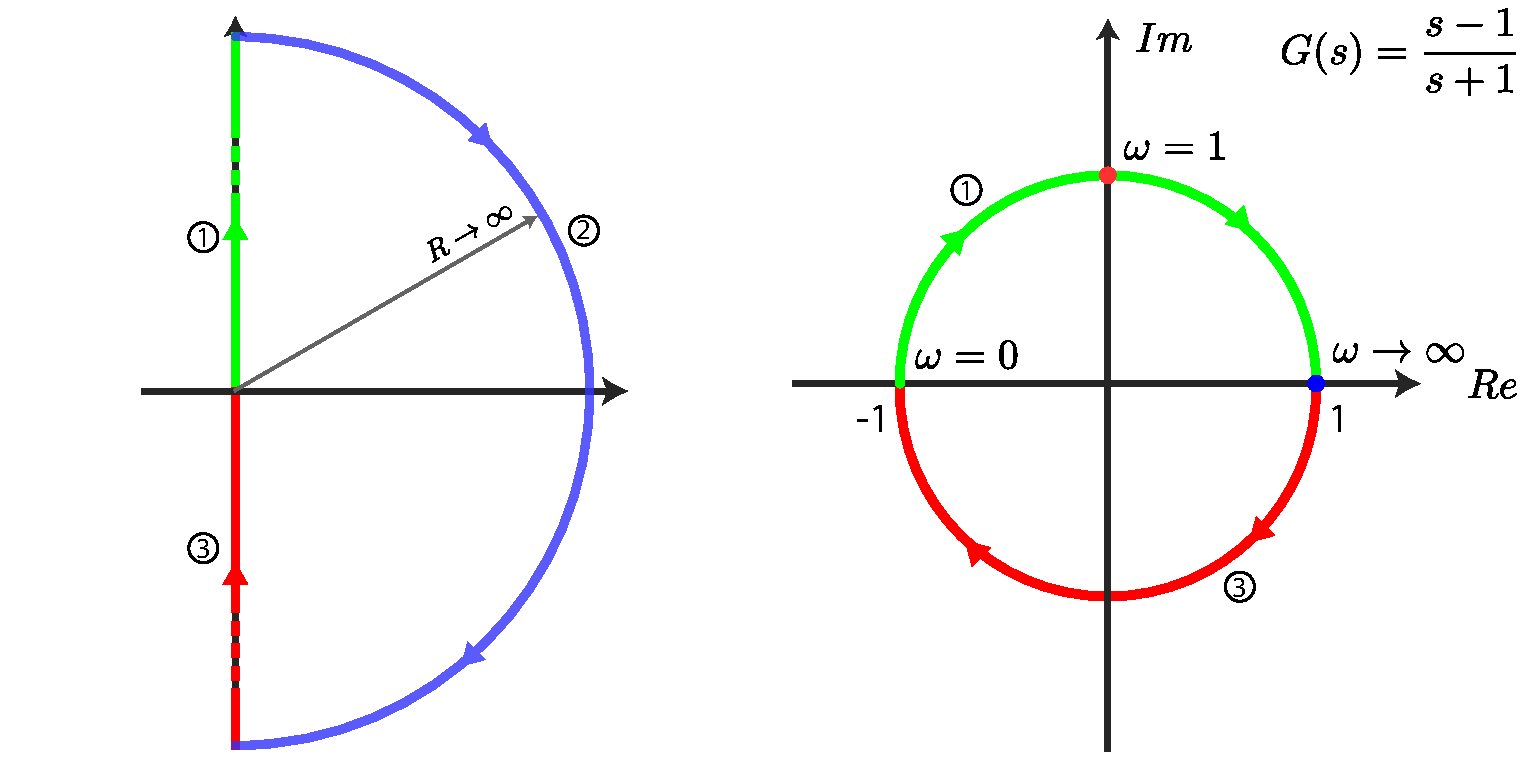
\includegraphics[width=0.9\textwidth]{ex1}
    \end{center}
  \end{minipage}

\vspace{6 pt}

We can see from the derived Nyquist plot that $N=1$, and 
we know that the system has 1 zero with positive real part 
$Z =1$. The total number of unstable poles is equal to
$P = Z - N = 1 - 1 = 0$, thus the system is obviously stable. 

\newpage

\textbf{Ex:} Let's analyze the feedforward stability of $G(s) =
\frac{1}{s+1}$ using Nyquist plot. 

\textbf{Solution:} Now let's analyze the Nyquist paths
%
\begin{enumerate}
  \item This is the polar plot that we covered in the previous
    lecture, where we plot $G(j \omega)$, where $\omega : 0 \to
    \infty$. In this case, the behavior when $\omega \to \infty$ is
    important. Now let's assume that $\omega \to R$ and $R \gg 1$
    % 
  \begin{align*}
   G_1(j R) &\approx \frac{1}{R^2} - \frac{1}{R} j
    \\
    \angle [ G_1(j \omega) ] &\approx -\pi / 2
   \end{align*}
%
  \item Now we should be careful with mapping the infinite radius
    circular path. Again let $s = R e^{j \theta}$ and $\theta : \pi/2
    \to -\pi/2$.  Then 
   we can derive that  
   \begin{align*}
     & G \left( R e^{j \theta} \right) = \approx \frac{1}{R e^{j
       \theta}} = \frac{e^{j (-\theta)}}{R}
       \\
    &\Rightarrow | G \left( R e^{j \theta} \right) | \approx \epsilon
      \ll 1
   \quad , \quad \angle [ G \left( R e^{j \theta} \right) ] \approx -\theta
   \end{align*}
   % 
   Note that when $\theta : \pi/2 \to -\pi/$, the infinite-small 
   contour around origin rotates in CCW direction. 
   %
   \item Last path (mapping of negative imaginaty axis) is again
   is the conjugate of polar plot with reverse direction. 
\end{enumerate}

If we follow the procedure, we obtain the following Nyquist plot. 

\vspace{6 pt}

  \begin{minipage}[h]{1\linewidth}
    \begin{center}
      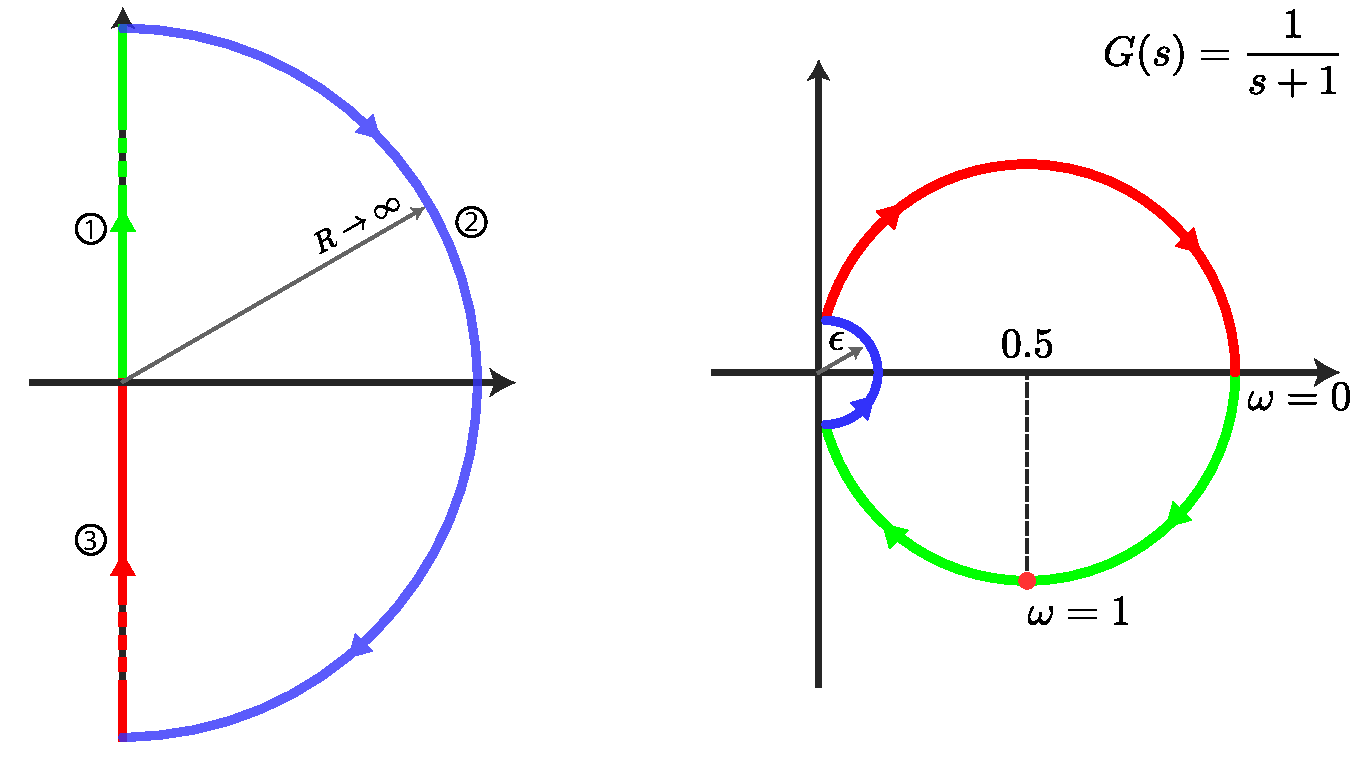
\includegraphics[width=0.9\textwidth]{ex2}
    \end{center}
  \end{minipage}

\vspace{6 pt}

We can see from the derived Nyquist plot that $N=0$, and 
we know that the system has no zero with positive real part 
$Z =0$. The total number of unstable poles is equal to
$P = Z - N = 0 - 0 = 0$, thus the system is obviously stable. 

\newpage

\textbf{Ex:} Analyze the feedforward stability of $G(s) =
\frac{1}{(s+1)^2}$ using Nyquist plot. 

\textbf{Solution:} Firs let's analyze the Nyquist paths
%
\begin{enumerate}
  \item This is the polar plot that we covered in the previous
    lecture, where we plot $G(j \omega)$, where $\omega : 0 \to
    \infty$. In this case, the behavior when $\omega \to \infty$ is
    important. Now let's assume that $\omega \to R$ and $R \gg 1$
    % 
  \begin{align*}
   G_1(j R) &\approx -\frac{1}{R^2} - \frac{1}{R^3} j
    \quad , \quad 
    \angle [ G_1(j \omega) ] \approx -\pi
   \end{align*}
%
  \item Again, we should be careful with mapping of  the infinite radius
    circular path. $s = R e^{j \theta}$ and $\theta : \pi/2 \to -\pi/2$.  Then 
   we can derive that  
   \begin{align*}
     & G \left( R e^{j \theta} \right) = \approx \frac{1}{R^2 e^{j
       2 \theta}} = \frac{e^{j (-2 \theta)}}{R^2}
       \\
    &\Rightarrow | G \left( R e^{j \theta} \right) | \approx
      \epsilon^2 \ll 1
   \quad , \quad \angle [ G \left( R e^{j \theta} \right) ] \approx -2
      \theta
   \end{align*}
   % 
   Note that when $\theta : \pi/2 \to -\pi/$, the infinite-small 
   contour around origin rotates in CCW direction. 
   %
   \item Last path (mapping of negative imaginaty axis) is again
   the conjugate of polar plot with reverse direction. 
\end{enumerate}

If we follow the procedure, we obtain the following Nyquist plot. 

\vspace{6 pt}

  \begin{minipage}[h]{1\linewidth}
    \begin{center}
      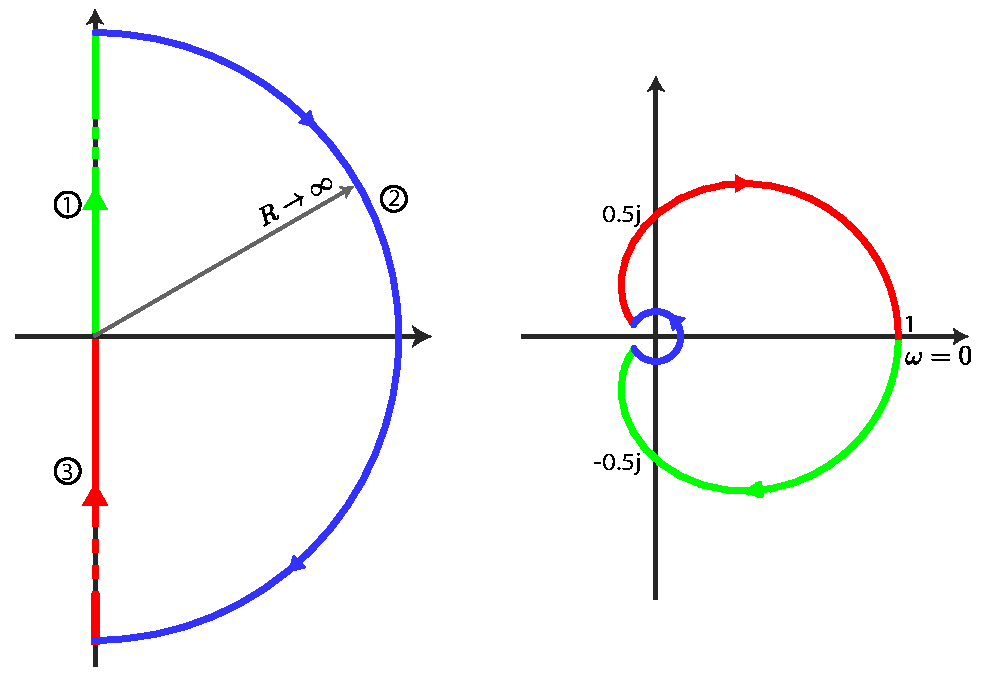
\includegraphics[width=0.9\textwidth]{ex3}
    \end{center}
  \end{minipage}

\vspace{6 pt}

We can see from the derived Nyquist plot that $N=0$, and 
we know that the system has no zero with positive real part 
$Z =0$. The total number of unstable poles is equal to
$P = Z - N = 0 - 0 = 0$, thus the system is obviously stable. 

\textbf{Ex:} Analyze the feedforward stability of $G(s) =
\frac{1}{(s+1)^3}$ using Nyquist plot. 

\textbf{Solution:} Firs let's analyze the Nyquist paths
%
\begin{enumerate}
  \item This is the polar plot that we have covered in the previous
    lecture, where we plot $G(j \omega)$, where $\omega : 0 \to
    \infty$. In this case, the behavior when $\omega \to \infty$ is
    important. Now let's assume that $\omega \to R$ and $R \gg 1$
    % 
  \begin{align*}
   G(j R) &\approx -\frac{3}{R^4} + \frac{1}{R^3} j
    \quad & \quad 
    \angle [ G(j \omega) ] &\approx \pi / 2
   \end{align*}
%
  \item Again, we should be careful with mapping of  the infinite radius
    circular path. $s = R e^{j \theta}$ and $\theta : \pi/2 \to -\pi/2$.  Then 
   we can derive that  
   \begin{align*}
     & G \left( R e^{j \theta} \right) = \approx \frac{1}{R^3 e^{j
       3 \theta}} = \frac{e^{j (-3 \theta)}}{R^3}
       \\
    &\Rightarrow | G \left( R e^{j \theta} \right) | \approx
      \epsilon^3 \ll 1
   \quad , \quad \angle [ G \left( R e^{j \theta} \right) ] \approx -3
      \theta
   \end{align*}
   % 
   Note that when $\theta : \pi/2 \to -\pi/$, the infinite-small 
   contour around origin rotates in CCW direction. 
   %
   \item Last path (mapping of negative imaginaty axis) is again
   the conjugate of polar plot with reverse direction. 
\end{enumerate}

If we follow the procedure, we obtain the following Nyquist plot. 

\vspace{6 pt}

  \begin{minipage}[h]{1\linewidth}
    \begin{center}
      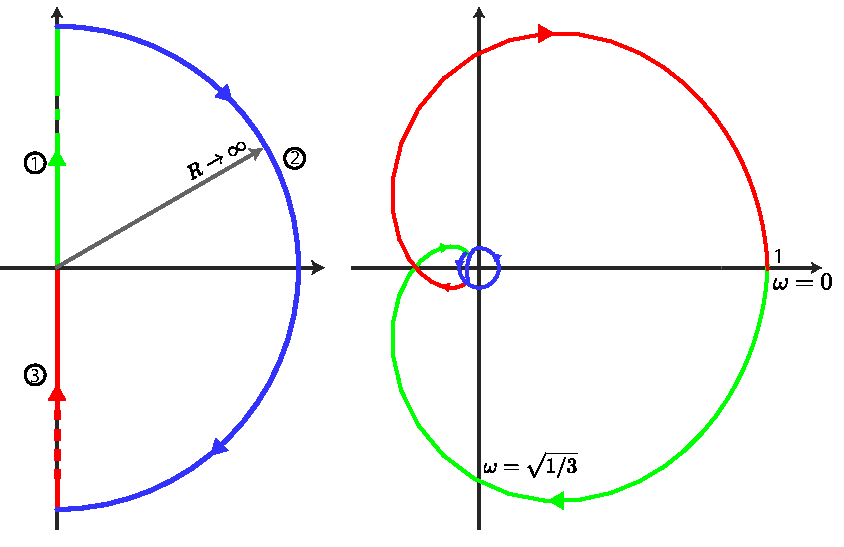
\includegraphics[width=0.99\textwidth]{ex4}
    \end{center}
  \end{minipage}

\vspace{6 pt}

If carefully analyze the encirclements around the origin, 
we can see that \textbf{net} encirclement around the origin is 
$N = 1 - 1$ (or $N = 2 - 2$). Based on this, we verify that   
the total number of unstable poles is equal to
$P = Z - N = 0 - 0 = 0$, thus the system is stable. 

\newpage

\textbf{Ex:} Analyze the feedforward stability of $G(s) =
\frac{1}{ (s-1)(s+ 2)}$ using Nyquist plot. 

\textbf{Solution:} In the polar plot we draw $G(j \omega)$ where $\omega : 0 \to \infty$
%
\begin{align*}
  G(j \omega) &= \frac{1}{ (j \omega - 1) (j \omega + 2) } = 
  \frac{-(j \omega + 1) (-j \omega + 2)}{ (\omega^2 + 1) (\omega^2 +
  4) } = \left[ -(2+\omega^2) - \omega j \right] \frac{1}{(\omega^2 + 1) (\omega^2 +
  4)}
\\
\forall \omega &\in (0 , \infty) , \ Re \lbrace G(j \omega)
  \rbrace < 0 \ \& \ Im \lbrace G(j \omega)
  \rbrace < 0
\end{align*}

Let's derive where the polar plot approachs when $\omega \to 0$
and $\omega \to \infty$
\begin{align*}
  \lim_{\omega \to 0} G(j \omega) &= -0.5 + 0 j
\\
  \lim_{\omega \to \infty} | G(j \omega) | &= 0
\quad , \quad
 \lim_{\omega \to \infty} \angle [ G(j \omega) ] = -\pi
\end{align*}

Now let's derive the Nyquist plot conditions for the infinite circle
on the Nyquist contour. In this path $s = R e^{j \theta}$ where $R \to
\infty$ (or $R \gg 1)$ and $\theta : \pi/2 \to - \pi/2$ (in CW
direction). Thus,
%
\begin{align*}
  G(R e^{j \theta}) &\approx \frac{1}{R^2 e^{j 2\theta}} =
  \frac{1}{R^2} e^{j (-2\theta)}
\\
  | G(R e^{j \theta}) | &\approx \epsilon \ll 1
\\
 \angle [ G(R e^{j \theta}) ] &= - 2 \theta \quad \theta : \pi/2 \to -\pi/2
\end{align*}
%
Note that associated Nyquist plot around origin turns approximatelly
$2 \pi$ radians in CCW direction. Last path is the mapping of negative imaginary axis which is simply
conjugate of the polar plot with reverse direction. 

\vspace{6 pt}

  \begin{minipage}[h]{1\linewidth}
    \begin{center}
      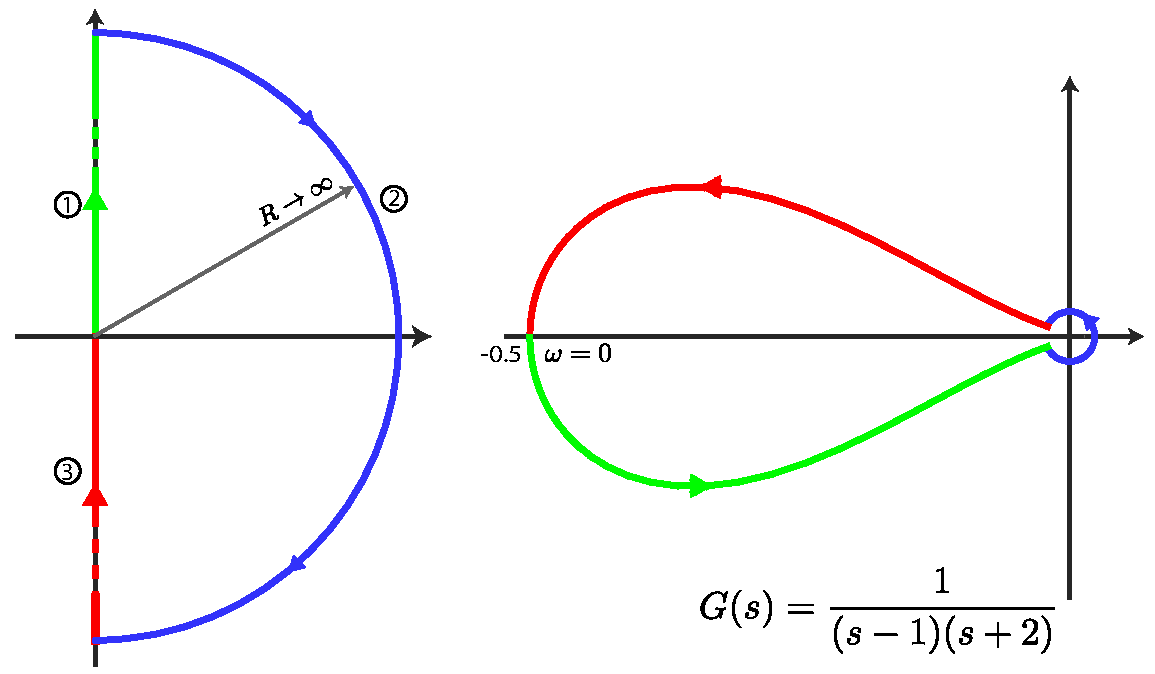
\includegraphics[width=0.98\textwidth]{ex5}
    \end{center}
  \end{minipage}

\vspace{6 pt}

If carefully analyze the encirclements around the origin, 
we can see that \textbf{net} CW encirclement around the origin is 
$N = - 1$. Based on this, we verify that   
the total number of unstable poles is equal to
$P = Z - N = 0 - (-1) = 1$, thus the system is indeed unstable. 


% **** This ENDS THE EXAMPLES. DON'T DELETE THE FOLLOWING LINE:
\end{document}